\documentclass[11pt,a4paper]{article}

\newcommand{\tumsoTime}{09:00 น. - 12:00 น.}
\newcommand{\tumsoRound}{1}

\usepackage{../tumso}

\begin{document}

\begin{problem}{สมบัติล้ำค่า}{standard input}{standard output}{1 seconds}{32 megabytes}{100}

บริษัทแห่งหนึ่งได้ทำการส่งสินค้าชิ้นหนึ่งผ่านทางรถไฟ โดยสินค้าชิ้นนั้นเป็นสมบัติที่ขุดพบภายในโบราณสถานแห่งหนึ่ง เพื่อนำไปค้นคว้าหาข้อมูลต่อไป

กลุ่มบุคคลกลุ่มหนึ่งได้รู้ถึงข้อมูลเหล่านี้จึงได้ขึ้นรถไฟเพื่อพยายามที่จะขโมยสมบัติ จนได้พบสมบัติที่ตามหา แต่ปัญหามีกระจกครอบสมบัติไว้จำนวน $t$ ชั้น มีแป้นกดตัวเลข $0-9$ และได้มีข้อความเขียนไว้ว่า 

"ถ้าอยากจะได้สมบัติไป จงแก้ปัญหาต่อไปนี้ มีแผ่นกระเบื้องสีขาวและสีดำขนาด $1*1$ อยู่ไม่จำกัดแผ่น ต้องการวางแผ่นกระเบื้องให้เป็นทางยาวขนาด $2*n$ โดยที่กระเบื้องสีดำห้ามวางอยู่ติดกันเด็ดขาด จะสามารถวางได้ทั้งหมดกี่วิธีที่แตกต่างกัน โดยให้ตอบเป็นเศษที่เกิดจากการหารคำตอบด้วย $98765431$"

เมื่อพวกเขาได้อ่านเลยคิดว่าคงเป็นไปไม่ได้ เพราะไม่รู้ $n$ เลยพยายามจะทำลายกระจก แต่มันก็ทนทานจนเกินไป จนได้สังเกตว่ารอบๆ โบกี้ที่บรรทุกสมบัติมีตัวเลขที่เป็นค่าของ $n$ ถูกเขียนเป็นจำนวน $t$ ค่า เลยรู้ได้ทันทีว่าต้องตอบทั้งหมด $t$ ครั้งกระจกจึงจะเปิดหมด เลยอยากให้คุณซึ่งเป็นโปรแกรมเมอร์คนเดียวในทีมแก้ปัญหานี้ เพื่อสมบัติที่อาจเป็นของล้ำค่าได้

\InputFile
บรรทัดที่ $1$ รับจำนวนเต็ม $t$ แสดงถึงจำนวนคำถาม $(1 \leq t \leq 10^3)$

บรรทัดที่ $2$ ถึง $t + 1$ รับจำนวนเต็ม $n_i$ $(1 \leq n_i \leq10^{18})$
\OutputFile
มีจำนวน $t$ บรรทัด ซึ่งบรรทัดที่ $i$ แสดงคำตอบของคำถามที่ $i$ 
\Scoring
ชุดทดสอบจะถูกแบ่งเป็น $3$ ชุด จะได้คะแนนในแต่ละชุดก็ต่อเมื่อโปรแกรมให้ผลลัพธ์ถูกต้องในชุดทดสอบย่อยทั้งหมด

\begin{description}

\item[ชุดที่ 1 (10 คะแนน)]  $1 \leq t \leq 15 , 1 \leq n_i \leq 15$ 

\item[ชุดที่ 2 (25 คะแนน)] $1 \leq t \leq 100 , 1 \leq n_i \leq 10^{6}$

\item[ชุดที่ 3 (65 คะแนน)] ไม่มีเงื่อนไขเพิ่มเติม

\end{description}

\Examples

\begin{example}
\exmp{3
1
2
4
}{3
7
41
}%
\exmp{7
12
15
14
4
3
14
5
}{47321
665857
275807
41
17
275807
99
}%
\end{example}

\Note
\begin{note}
ยกตัวอย่างกรณีที่ $n = 2$ สามารถวางได้ 7 แบบที่แตกต่างกันดังนี้

\begin{center}
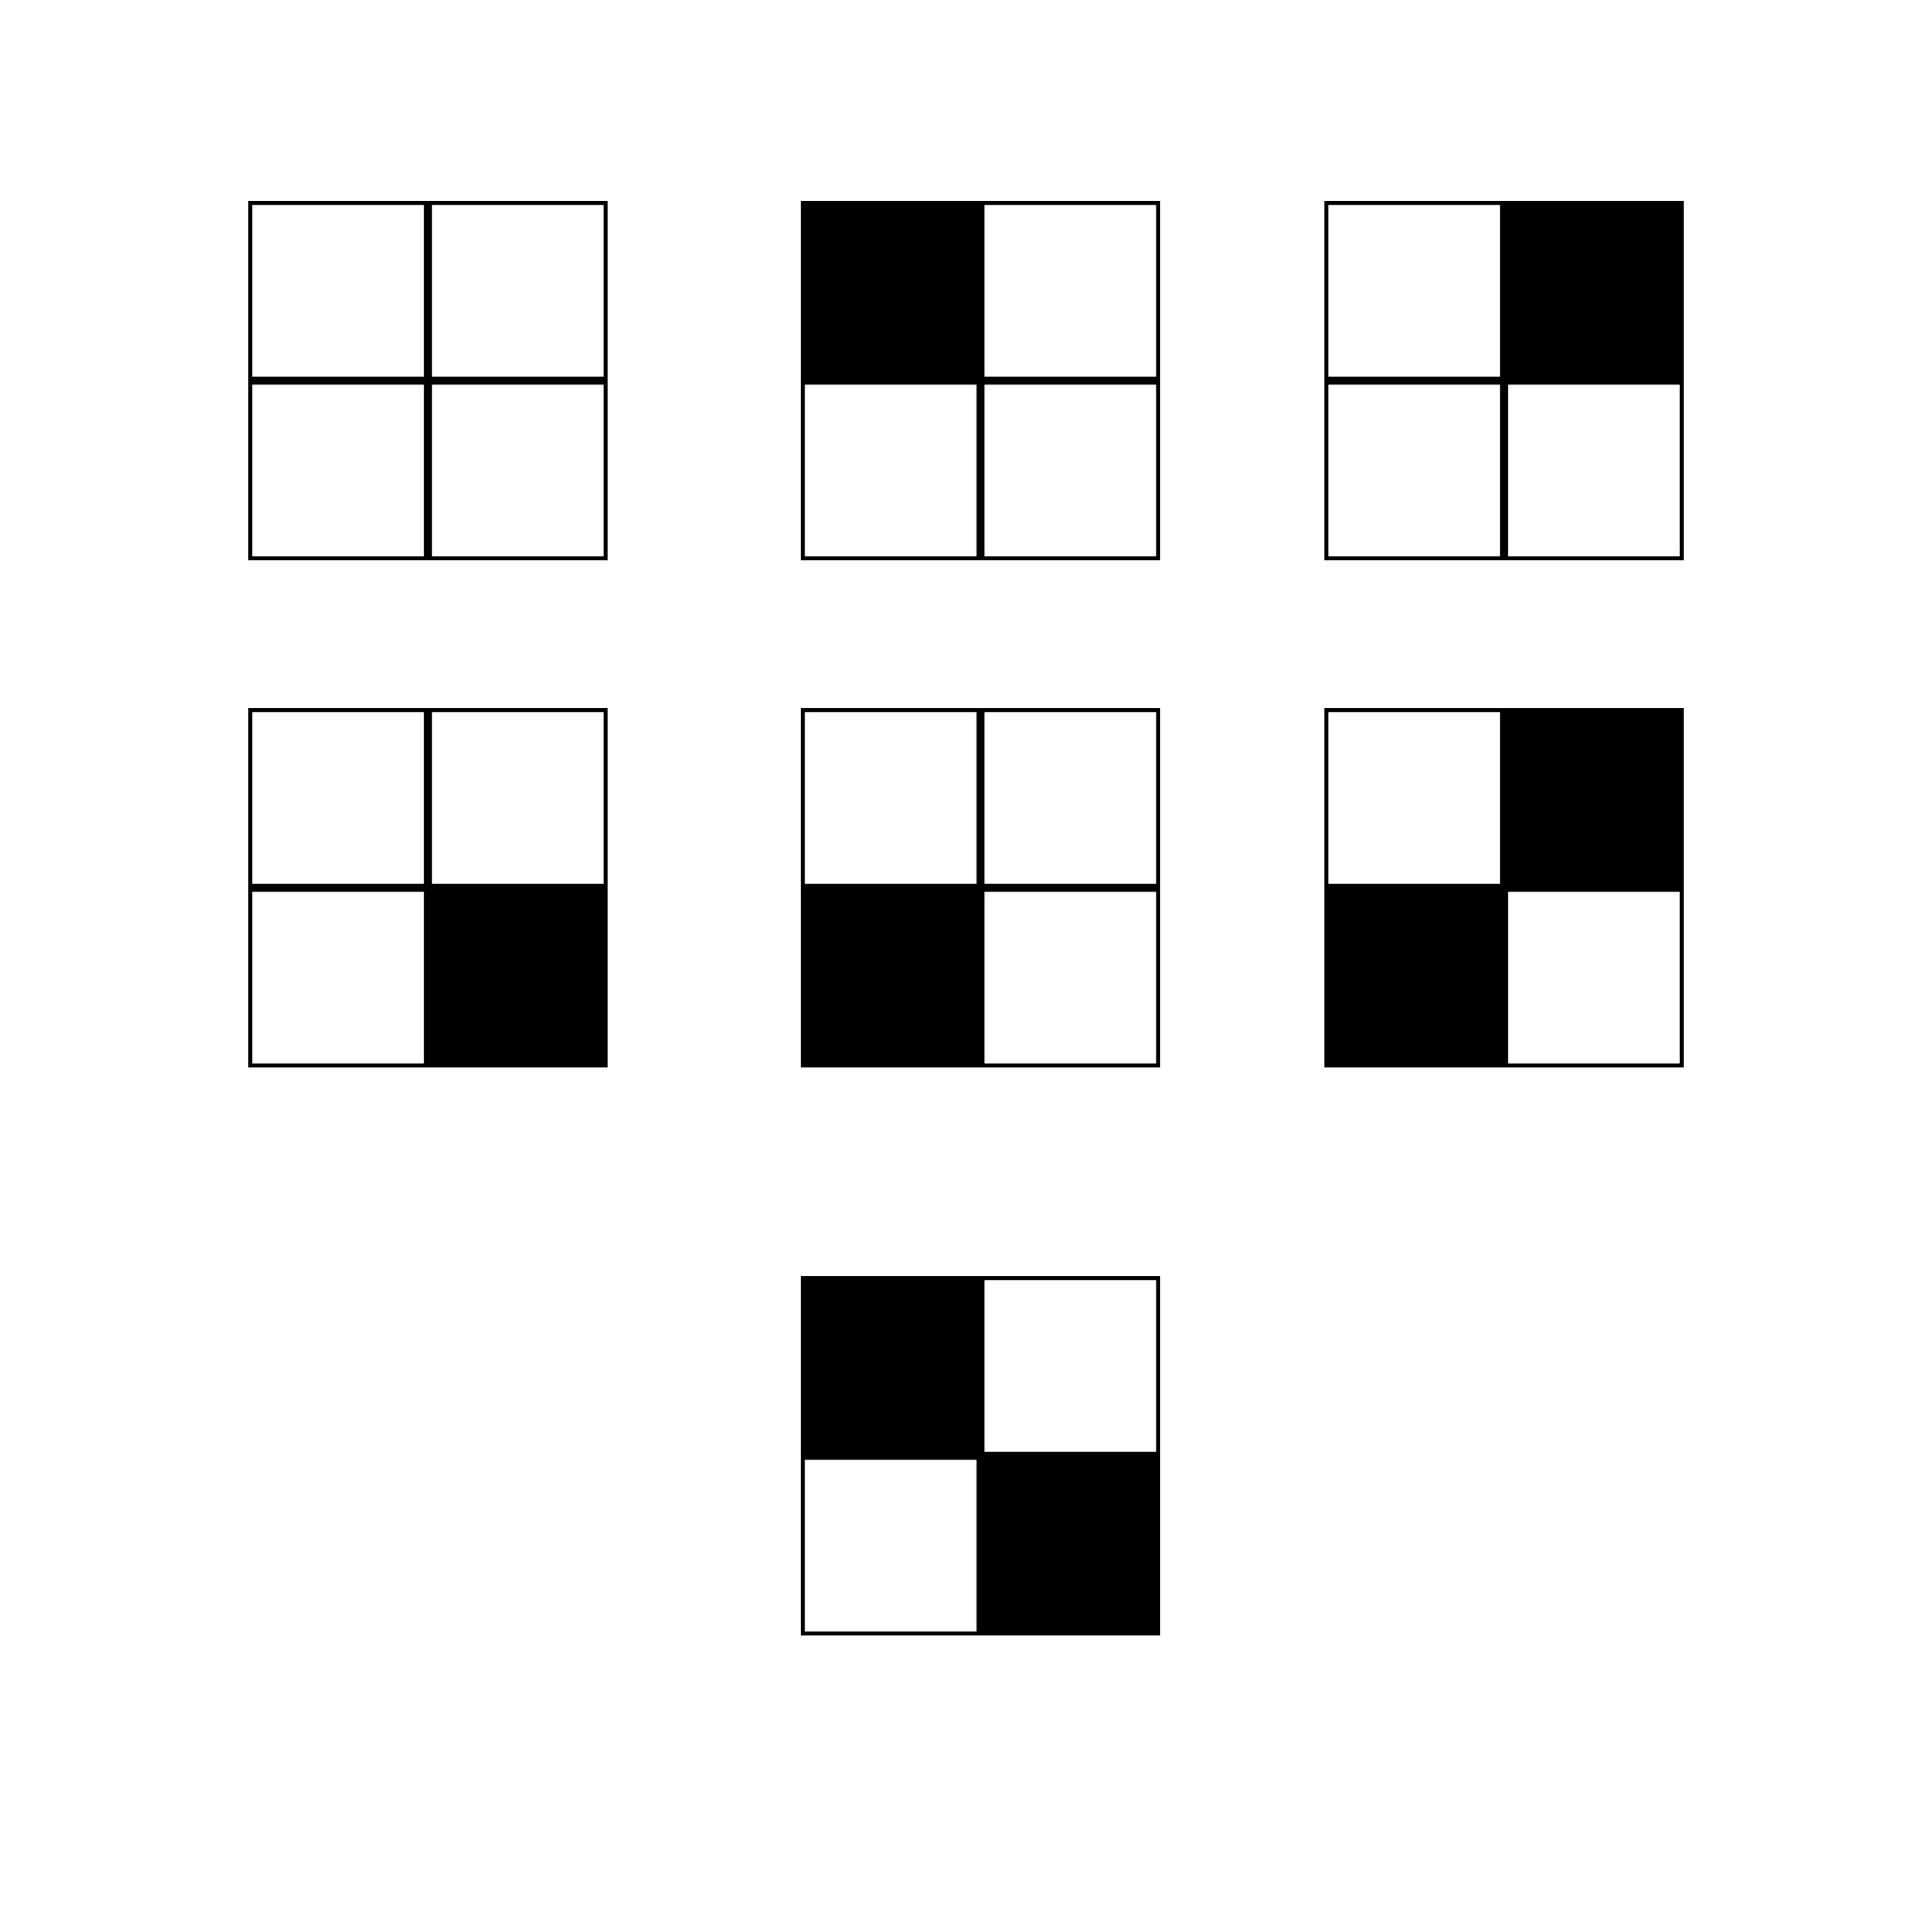
\includegraphics[width=8cm]{Sample.jpg}
\end{center}

\end{note}

\end{problem}

\end{document}
